\documentclass[a4paper, 12pt]{article}%тип документа

%отступы
\usepackage[left=2cm,right=2cm,top=2cm,bottom=3cm,bindingoffset=0cm]{geometry}

%Русский язык
\usepackage[T2A]{fontenc} %кодировка
\usepackage[utf8]{inputenc} %кодировка исходного кода
\usepackage[english,russian]{babel} %локализация и переносы

%Вставка картинок
\usepackage{wrapfig}
\usepackage{graphicx}
\graphicspath{{pictures/}}
\DeclareGraphicsExtensions{.pdf,.png,.jpg}

%оглавление
\usepackage{titlesec}
\titlespacing{\chapter}{0pt}{-30pt}{12pt}
\titlespacing{\section}{\parindent}{5mm}{5mm}
\titlespacing{\subsection}{\parindent}{5mm}{5mm}
\usepackage{setspace}

%Графики
\usepackage{multirow}
\usepackage{pgfplots}
\pgfplotsset{compat=1.9}

%Математика
\usepackage{amsmath, amsfonts, amssymb, amsthm, mathtools}

%Заголовок
\author{Валеев Рауф Раушанович \\
группа 825}
\title{\textbf{Работа 5.1.2\\
Эффект Комптона}}
\newtheorem{task}{Задача}
\begin{document}
\maketitle
\newpage
\paragraph{Цель работы:} С помощью сцинтилляционного спектрометра исследуется энергетический спектр $\gamma$ - квантов, рассеянных на графите. Определяется энергия рассеянных $\gamma$ -квантов в зависимости от угла рассеяния, а также энергия покоя частиц, на которых происходит комптоновское рассеяние.

\section{Теория}
Рассеяние $\gamma$ -лучей в веществе относится к числу явлений, в которых особенно ясно проявляется двойственная природа излучения. Волновая теория, хорошо объясняющая рассеяние длинноволнового иЗлучения, испытывает трудности при описании рассеяния рентгеновских и $\gamma$ -лучей. Эта теория, в частности, не может объяснить, почему в составе рассеянного излучения, измеренного Комптоном, кроме исходной волны с частотой $\omega_{0}$ появляется дополнительная длинноволновая компонента, отсутствующая в спектре первичного излучения.

Появление этой компоненты легко объяснимо, если считать, что $\gamma$-излучение представляет собой поток квантов (фотонов), имеющих энергию $\hbar \omega$ и импульс $p=\hbar \omega / c .$ Эффект Комптона - увеличение длины волны рассеянного излучения по сравнению с падающим - интерпретируется как результат упругого соударения двух частиц: $\gamma$ -кванта (фотона) и свободного электрона.

Рассмотрим элементарную теорию эффекта Комптона. Пусть электрон до соударения покоился (его энергия равна энергии покоя $m c^{2}$ ), a $\gamma$ -квант имел начальную энергию $\hbar \omega_{0}$ и импульс $\hbar \omega_{0} / c .$ После соударения электрон приобретает энергию $\gamma m c^{2}$ и импульс $\gamma m v,$ где $\gamma=$ $=\left(1-\beta^{2}\right)^{-1 / 2}, \beta=v / c,$ a $\gamma$ -квант рассеивается на некоторый угол $\theta$ по отношению к первоначальному направлению движения. Энергия и импульс $\gamma$ -кванта становятся соответственно равным и $\hbar \omega_{1}$ и $\hbar \omega_{1} / c($ рис. 1$)$. Запишем для рассматриваемого процесса законы сохранения энергии и импульса:
$$
\begin{array}{c}
m c^{2}+\hbar \omega_{0}=\gamma m c^{2}+\hbar \omega_{1} \\
\frac{\hbar \omega_{0}}{c}=\gamma m v \cos \varphi+\frac{\hbar \omega_{1}}{c} \cos \theta \\
\gamma m v \sin \varphi=\frac{\hbar \omega_{1}}{c} \sin \theta
\end{array}
$$
Решая совместно эти уравнения и переходя от частот $\omega_{0}$ и $\omega_{1}$ к длинам волн $\lambda_{0}$ и $\lambda_{1},$ нетрудно получить, что изменение длины волны рассеянного излучения равно
\begin{equation}
\Delta \lambda=\lambda_{1}-\lambda_{0}=\frac{h}{m c}(1-\cos \theta)=\Lambda_{\mathrm{K}}(1-\cos \theta)
\end{equation}
где $\lambda_{0}$ и $\lambda_{1}$ - длины волн $\gamma$ -кванта до и после рассеяния, а величина
$$
\Lambda_{\mathrm{K}}=\frac{h}{m c}=2,42 \cdot 10^{-10} \mathrm{cm}
$$

Основной целью данной работы является проверка соотношения
(1). Применительно к условиям нашего опыта формулу
(1) следует преобразовать от длин волн к энергии $\gamma$ -квантов. Как нетрудно показать, соответствующее выражение имеет вид
\begin{equation}
\frac{1}{\varepsilon(\theta)}-\frac{1}{\varepsilon_{0}}=1-\cos \theta
\end{equation}
Здесь $\varepsilon_{0}=E_{0} /\left(m c^{2}\right)-$ выраженная в единицах $m c^{2}$ энергия $\gamma$ -квантов, падаюших на рассеиватель, $\varepsilon(\theta)$ - выраженная в тех же единицах энергия квантов, испытавших комптоновское рассеяние на угол $\theta, m-$ масса электрона.


\section{Экспериментальная установка}
Блок-схема установки изображена на рис. $3 .$ Источником излучения 1 служит $137 \mathrm{Cs},$ испускаюший $\gamma$ -лучи с энергией 662 кэВ. Он помещен в толстостенный свинцовый контейнер с коллиматором. Сформированный коллиматором узкий пучок $\gamma$ -квантов попадает на графитовую мишень 2 (цилиндр диаметром 40 мм и высотой 100 мм).

\begin{figure}[h]
\begin{center}
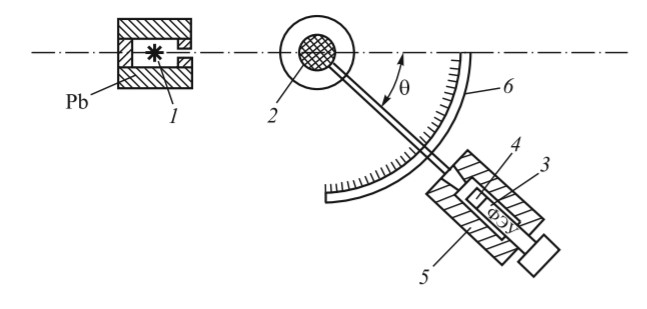
\includegraphics[width = \textwidth]{16.jpg}
\caption{Экспериментальная установка}
\end{center}
\end{figure}

Кванты, испытавшие комптоновское рассеяние в мишени, регистрируются сцинтилляционным счетчиком, принцип работы которого рассмотрен в работе 5.3. Счетчик состоит из фотоэлектронного умножителя 3 (далее ФЭУ) и сцинтиллятора $4^{*}$ ). Сцинтиллятором служит кристалл NaI(Tl) цилиндрической формы диаметром 40 мм и высотой 40 мм, его выходное окно находится в оптическом контакте с фотокатодом ФЭУ. Сигналы, возникающие на аноде ФЭУ, подаются на ЭВМ для амплитудного анализа. Кристалл и ФЭУ расположены в светонепроницаемом блоке, укрепленном на горизонтальной штанге. Штанга вместе с этим блоком может вращаться относительно мишени, угол поворота отсчитывается по лимбу $6 .$


\section{Обработка результатов}

Для обработки результатов используется формула $(2)$ с замененными энергиями квантов на $N(\theta)$.
\begin{equation}
\frac{1}{N(\theta)} - \frac{1}{N(0)} = A(1-\cos\theta)
\end{equation}
\newpage
\section{Ход работы}
Для начала сделаем проверку того, что при увеличении угла фотопик смещается влево (то есть того, что оборудование исправно и что данные, которые мы получаем, хотя бы качественно, соответствуют эффекту Комптона в данном случае).
\begin{figure}[h]
\begin{center}
\begin{minipage}[h]{0.4\linewidth}
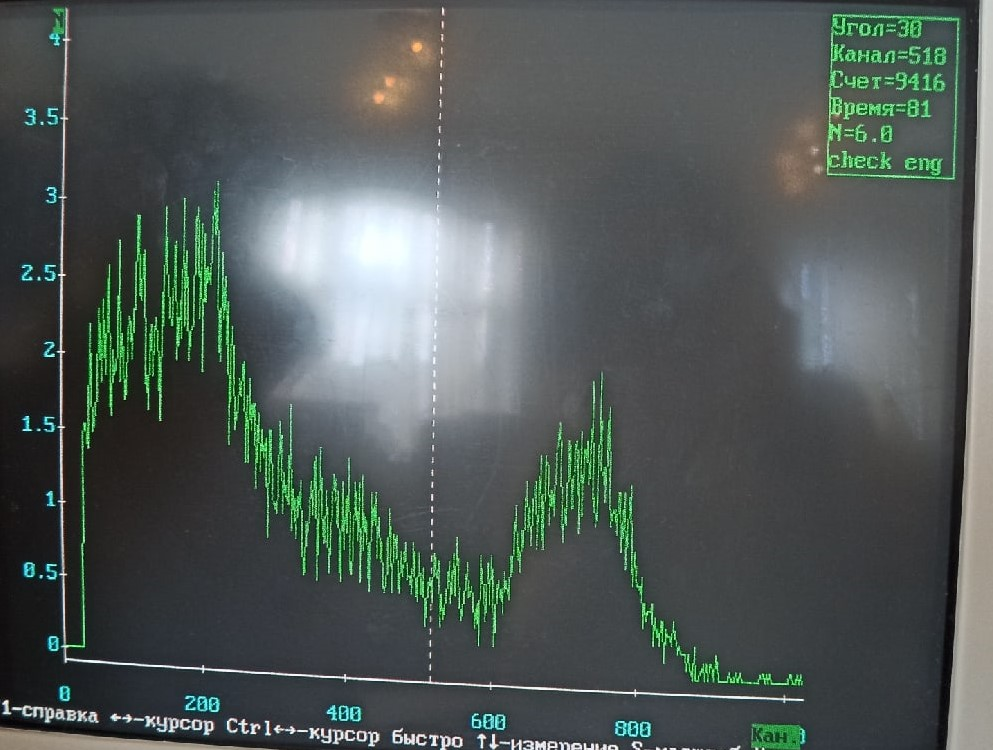
\includegraphics[width=1\linewidth]{2.jpg}
\caption{Проверка для $\theta = 30^0$} 
\end{minipage}
\hfill
\begin{minipage}[h]{0.45\linewidth}
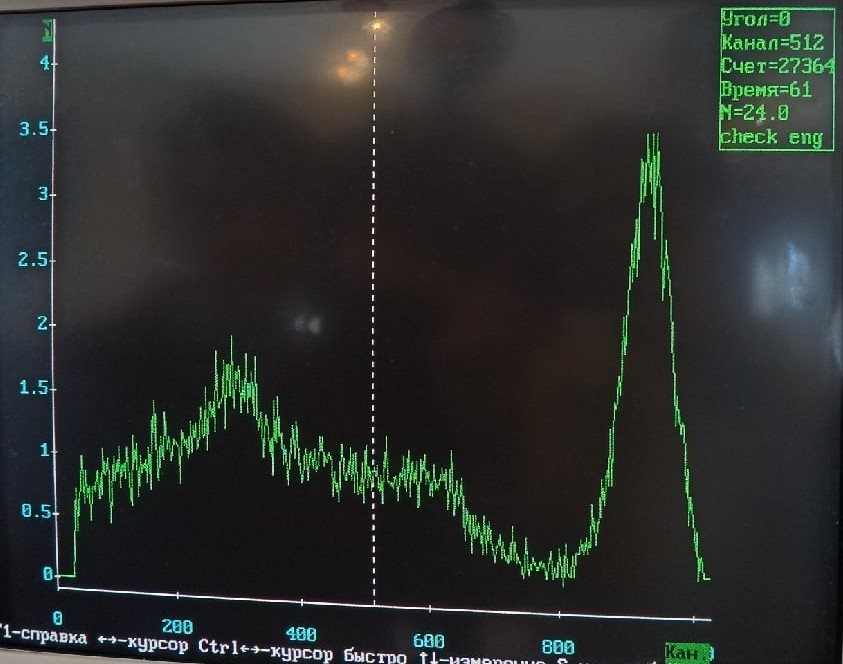
\includegraphics[width=1\linewidth]{3.jpg}
\caption{Проверка для $\theta = 0^0$} 
\end{minipage}
\end{center}
\end{figure}

Далее, устанавливая сцинтилляционный датчик под разными углами мы получаем картины пиков, по которым мы измеряем уже номера каналов, в которых пик.

Ниже приведены сами графики, которые мы получали.

\begin{figure}[h]
\begin{minipage}[h]{0.3\linewidth}
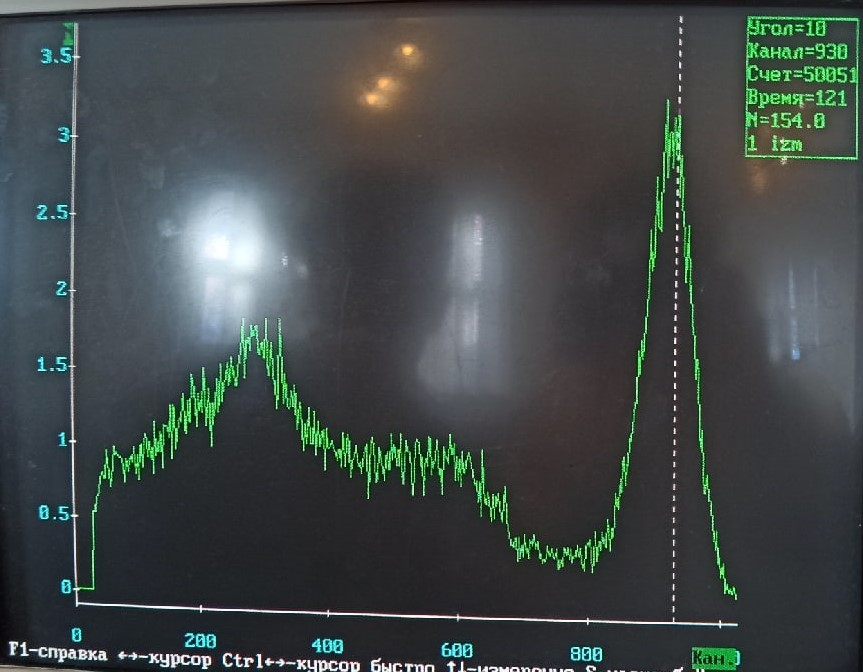
\includegraphics[width = 1\linewidth]{4.jpg}
\caption{$\theta = 10^0$}
\end{minipage}
\hfill
\begin{minipage}[h]{0.3\linewidth}
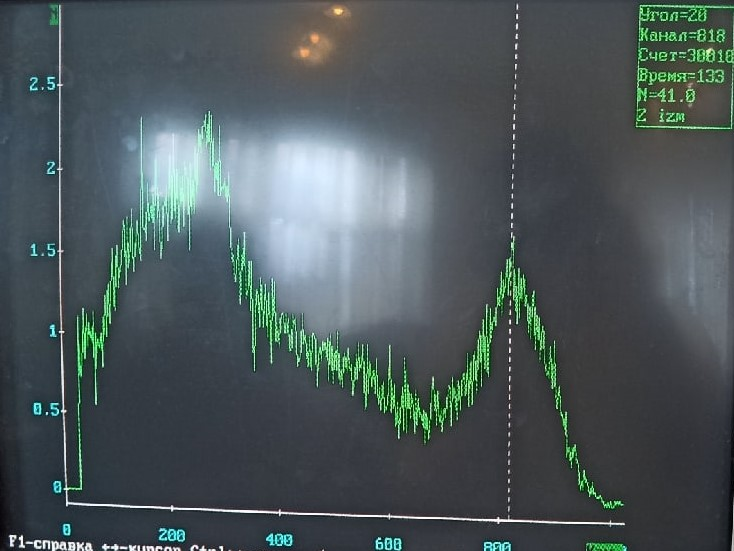
\includegraphics[width = 1\linewidth]{5.jpg}
\caption{$\theta = 20^0$}
\end{minipage}
\hfill
\begin{minipage}[h]{0.3\linewidth}
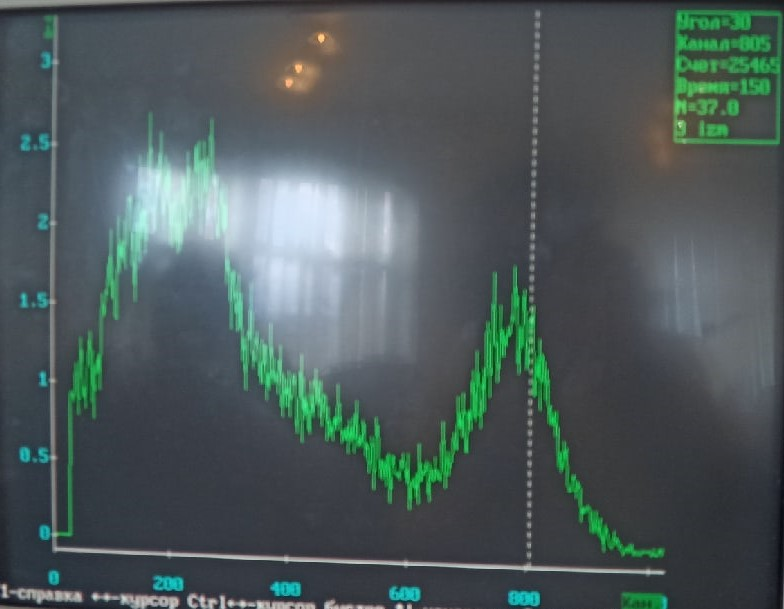
\includegraphics[width = 1\linewidth]{6.jpg}
\caption{$\theta = 30^0$}
\end{minipage}
\end{figure}
\begin{figure}[h]
\begin{minipage}[h]{0.3\linewidth}
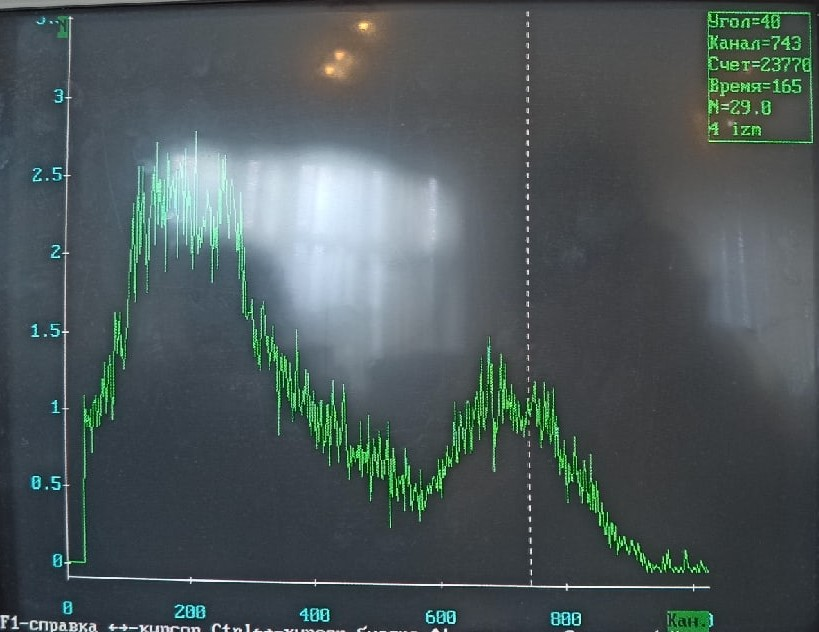
\includegraphics[width = 1\linewidth]{7.jpg}
\caption{$\theta = 40^0$}
\end{minipage}
\hfill
\begin{minipage}[h]{0.3\linewidth}
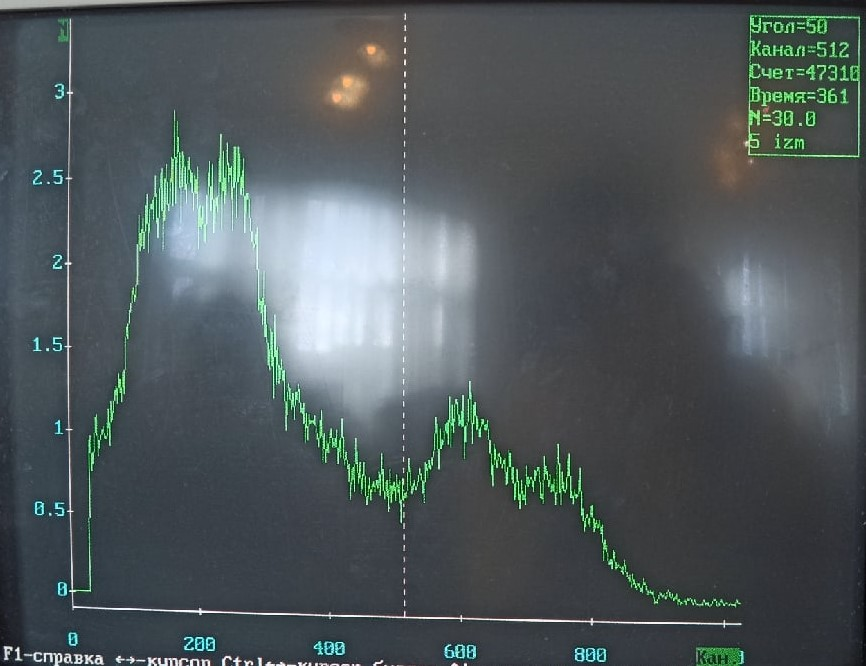
\includegraphics[width = 1\linewidth]{8.jpg}
\caption{$\theta = 50^0$}
\end{minipage}
\hfill
\begin{minipage}[h]{0.3\linewidth}
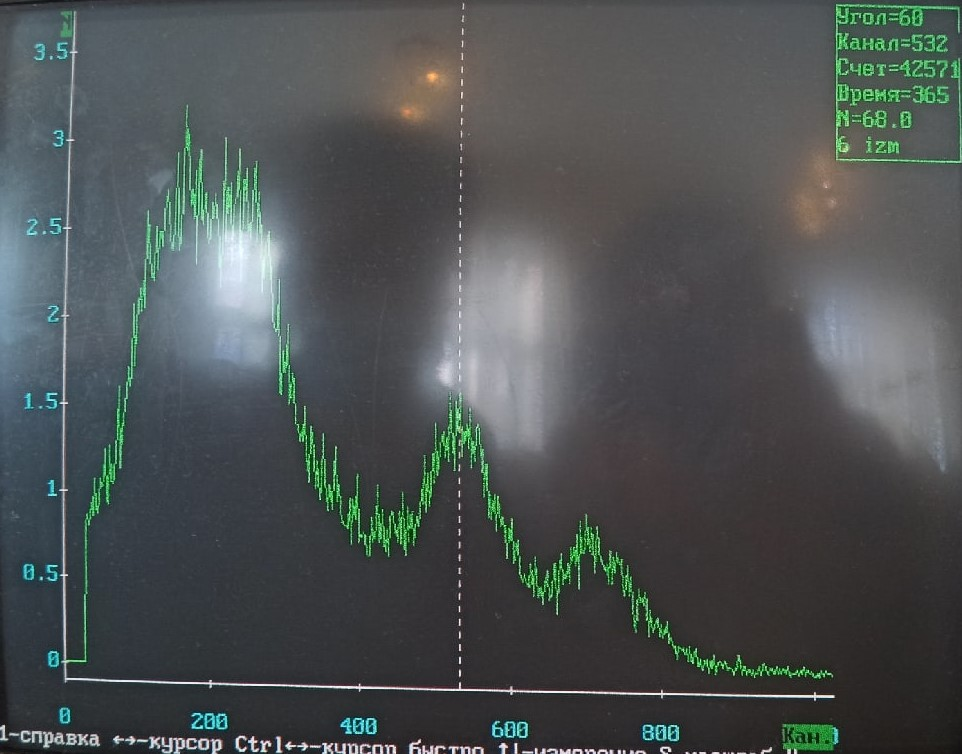
\includegraphics[width = 1\linewidth]{9.jpg}
\caption{$\theta = 60^0$}
\end{minipage}
\end{figure}
\begin{figure}[h]
\begin{minipage}[h]{0.3\linewidth}
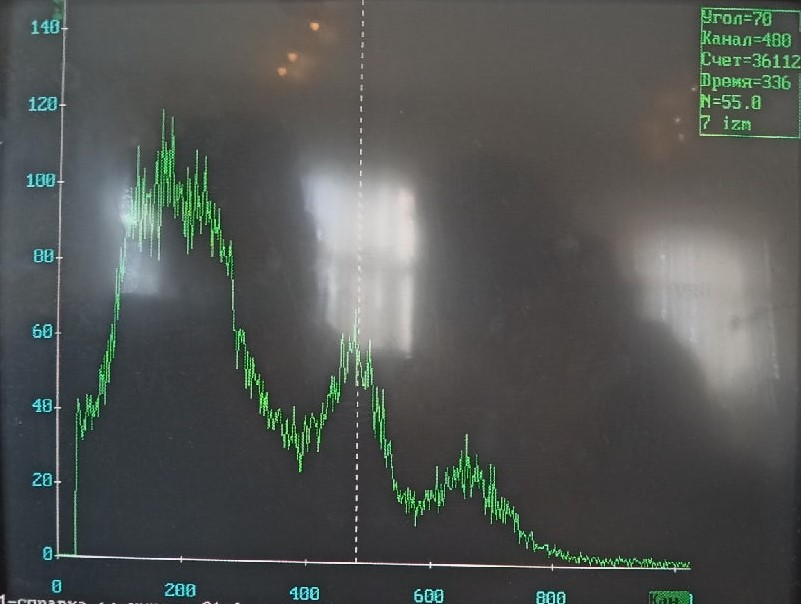
\includegraphics[width = 1\linewidth]{10.jpg}
\caption{$\theta = 70^0$}
\end{minipage}
\hfill
\begin{minipage}[h]{0.3\linewidth}
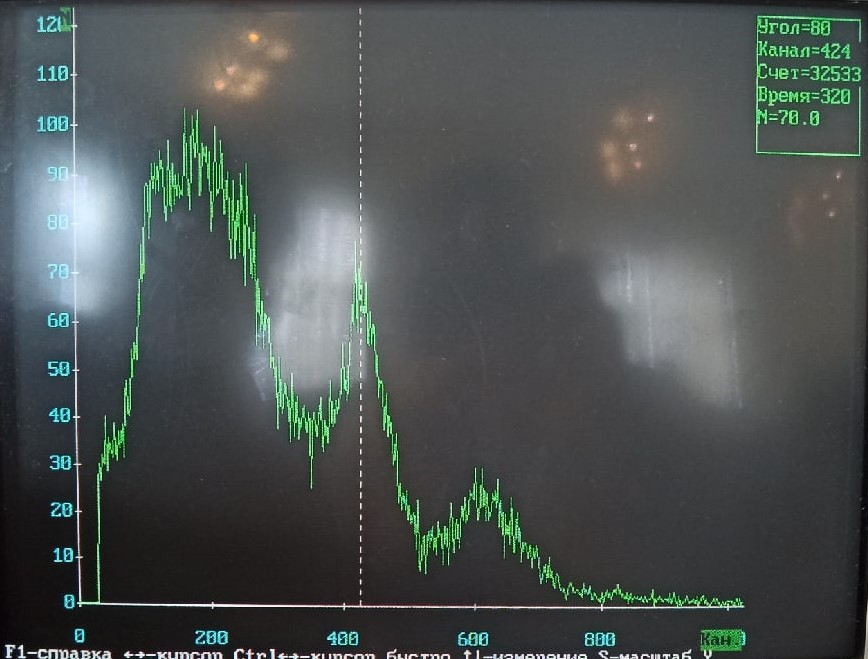
\includegraphics[width = 1\linewidth]{11.jpg}
\caption{$\theta = 80^0$}
\end{minipage}
\hfill
\begin{minipage}[h]{0.3\linewidth}
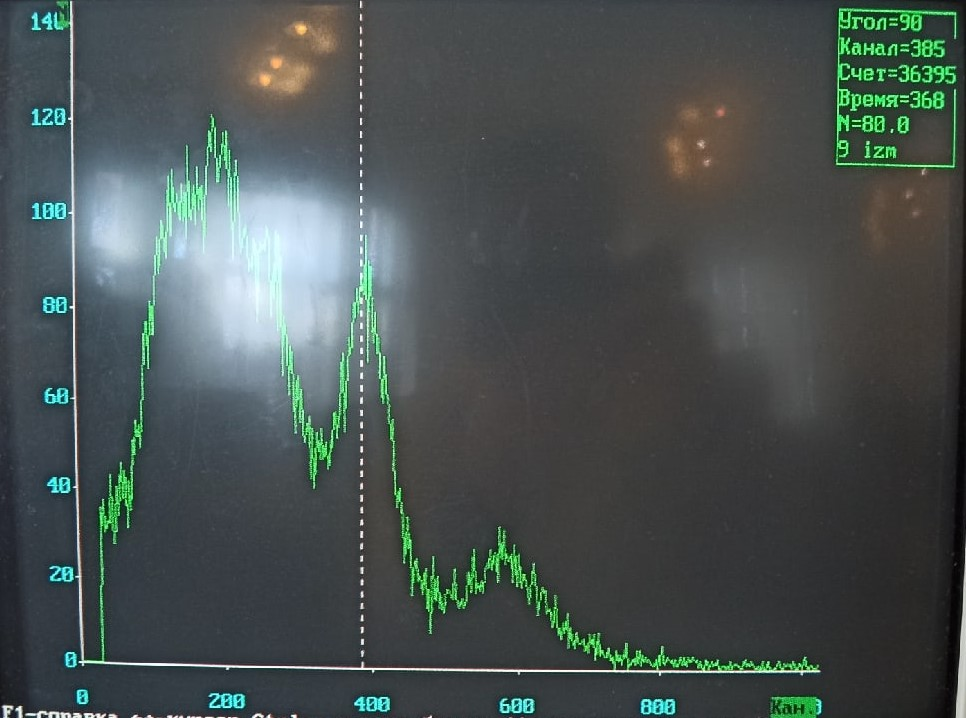
\includegraphics[width = 1\linewidth]{12.jpg}
\caption{$\theta = 90^0$}
\end{minipage}
\end{figure}
\begin{figure}[h]
\begin{minipage}[h]{0.3\linewidth}
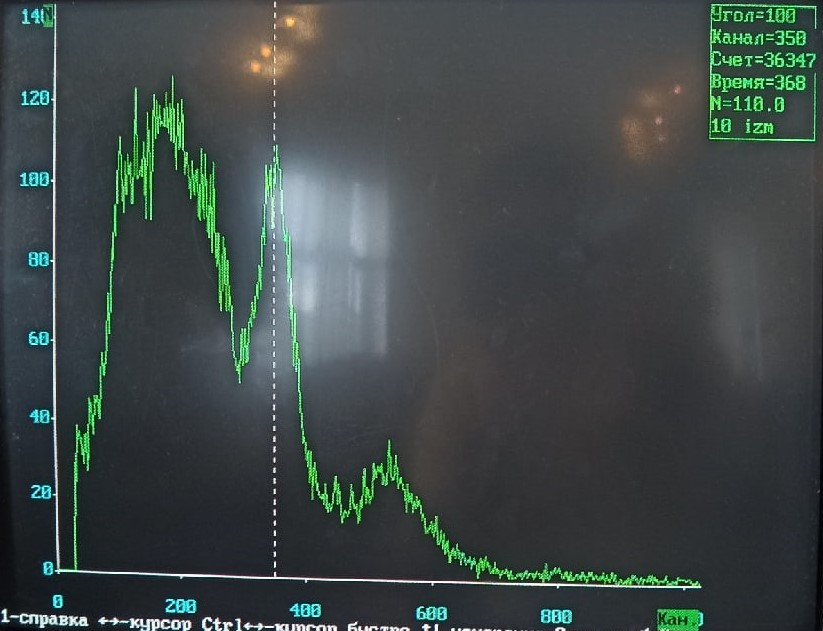
\includegraphics[width = 1\linewidth]{13.jpg}
\caption{$\theta = 100^0$}
\end{minipage}
\hfill
\begin{minipage}[h]{0.3\linewidth}
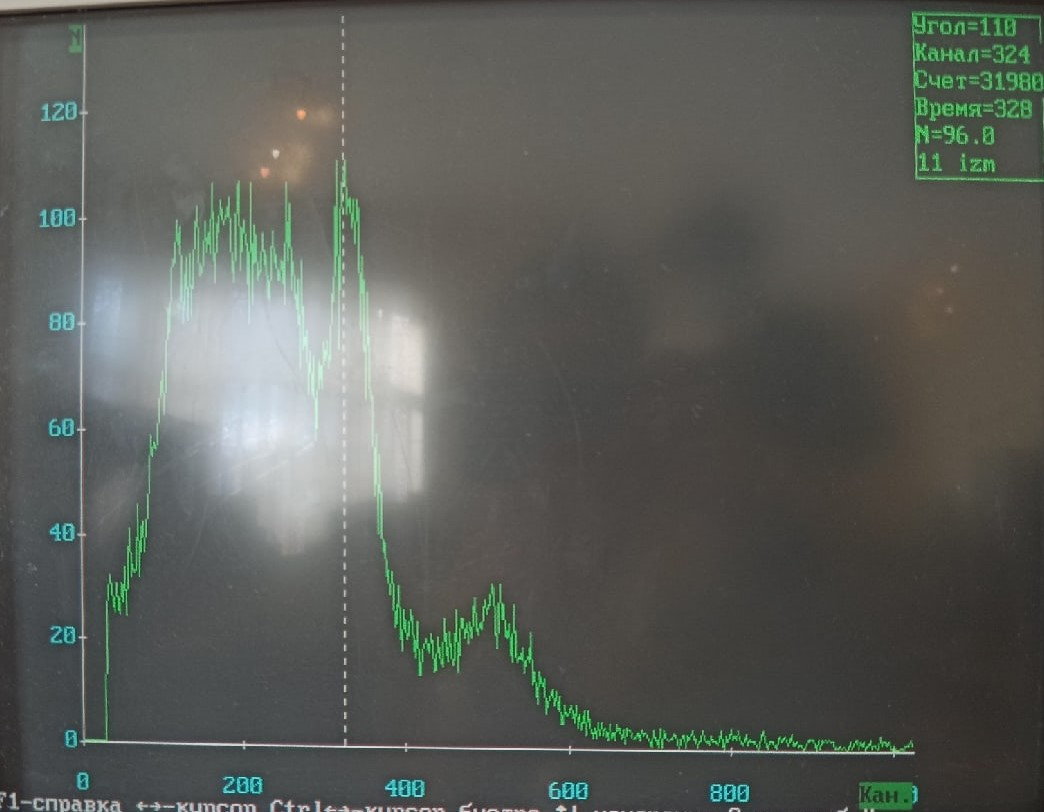
\includegraphics[width = 1\linewidth]{14.jpg}
\caption{$\theta = 110^0$}
\end{minipage}
\hfill
\begin{minipage}[h]{0.3\linewidth}
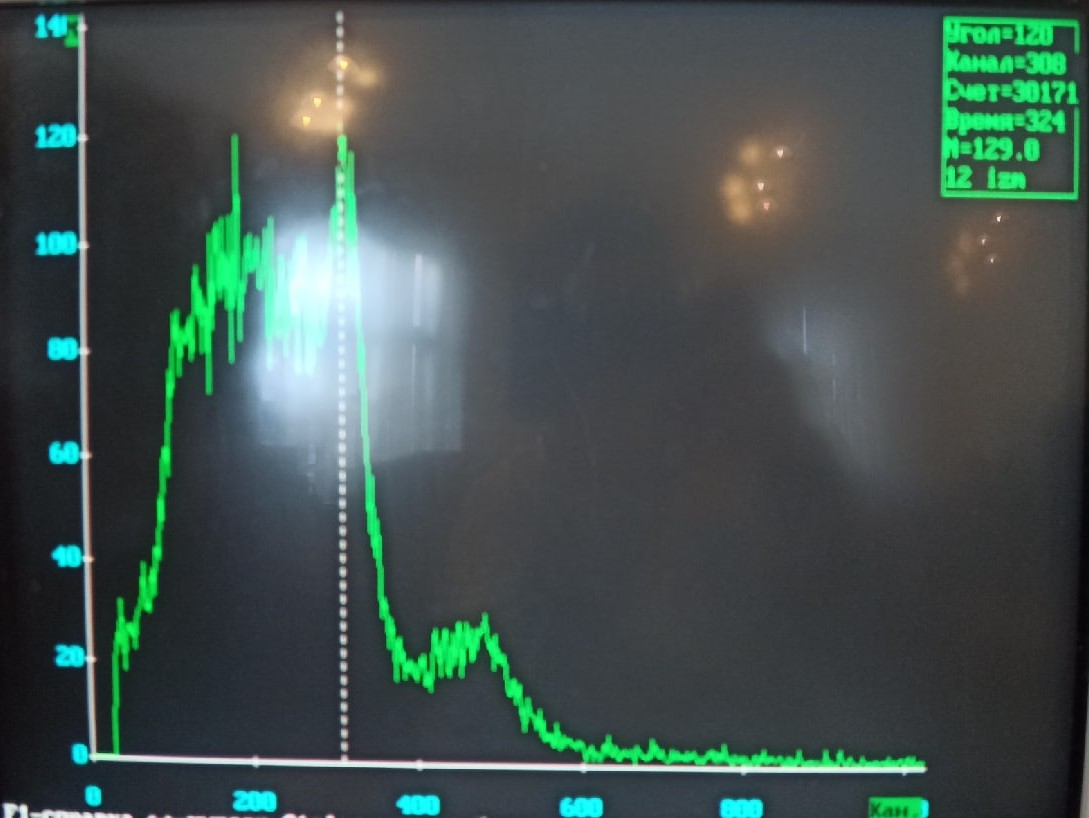
\includegraphics[width = 1\linewidth]{15.jpg}
\caption{$\theta = 120^0$}
\end{minipage}
\end{figure}

На последних графиках мы видим некую аномалию в видах графиков, поскольку и нас возникает как будто бы третий пик. На самом деле, если мы будем мерять номер канала, на котором он находится, то мы увидим, что это не пик фотоэффекта. Я предполагаю, что это из-за того, что часть графика находится ниже, чем должна быть. Это может быть связано с тем, что наш материал, на котором рассеиваются $\gamma$-кванты не идеален. Он может быть не идеально однородным, или не круглым по форме, из-за чего, при увеличении угла, мы видим данную аномалию. Очевидно, что при увеличении времени измерения до нескольких часов ушла бы даже эта аномалия, но в рамках лабораторного практикума это не представляется возможным.

Далее, мы приступим к проверке соотношения $(3)$, коэффициент $A$ найдем с помощью графика зависимости $1-\cos \theta$ от $\frac{1}{N(\theta)} - \frac{1}{N(0)}$. В таблице занесены все измеренные величины и процесс проверки соотношения (приведена после графика).

Теперь поговорим о погрешностях всех величин, которые мы видим ниже в таблице:
\begin{enumerate}
\item Для угла за погрешность мы берем просто половину цены деления шкалы, то есть $1 ^0$
\item Для номера пика погрешность ищем как полуширину интервала, в котором сам пик достигается. Так как после этого график достаточно быстро убывает (если смотреть относительно максимума), этого будет вполне достаточно
\item Для того, чтобы график был характерный для нашего эксперимента, при увеличении угла мы так же увеличиваем время, в течении которого проводим один эксперимент. Это сделано из-за того, что при увеличении угла падает интенсивность квантов, из-за чего при измерении за малый промежуток времени увеличивается влияние внешних источников и флуктуации направления квантов. Для этого оно и приведено.
\item Погрешность $\frac{1}{N(\theta)} - \frac{1}{N(0)}$ считаем по формуле
\[\sigma_{\frac{1}{N(\theta)} - \frac{1}{N(0)}} = \left(\frac{1}{N(\theta)} - \frac{1}{N(0)}\right) \cdot \sqrt{\frac{\sigma^2_{N(0)}}{N^6(0)} + \frac{\sigma^2_{N(\theta)}}{N^6(\theta)}}\]
\item Погрешность $1-\cos \theta$ считаем по формуле
\[\sigma_{1-\cos\theta} = \left(1-\cos\theta\right) \left| \frac{\sin\theta}{\theta} \sigma_{\theta}\right|\]
\item Погрешность $A(1-\cos\theta)$ считаем по формуле
\[\sigma_{A(1-\cos\theta)} = A(1-\cos\theta)\sqrt{\frac{\sigma^2_A}{A^2} + \frac{\sigma^2_{1-\cos\theta}}{(1-\cos\theta)^2}}\]
\item Погрешность $f = \frac{A(1-\cos\theta)}{\frac{1}{N(\theta)} - \frac{1}{N(0)}}$ считаем по формуле
\[\sigma_f = f \sqrt{\frac{\sigma_{A(1-\cos\theta)}^2}{(1-\cos\theta)^2} + \frac{\sigma_{\frac{1}{N(\theta)} - \frac{1}{N(0)}}^2}{\left(\frac{1}{N(\theta)} - \frac{1}{N(0)}\right)^2}}\]
\end{enumerate}

\begin{figure}[h]
\begin{center}
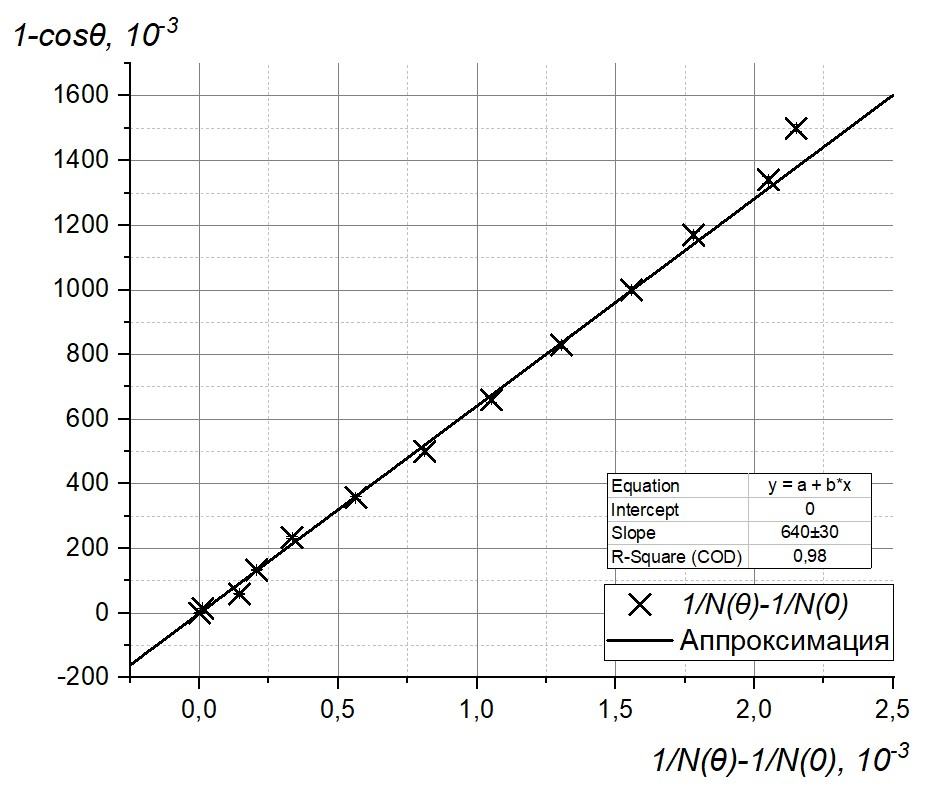
\includegraphics[width = 0.75\textwidth]{1.jpg}
\caption{График зависимости $1-\cos \theta$ от $\frac{1}{N(\theta)} - \frac{1}{N(0)}$
}
\end{center}
\end{figure}
\newpage
\begin{table}[h!]
\begin{center}
\begin{tabular}{|c|c|c|c|c|}
\hline
$\theta$, $^0$ & $\sigma_{\theta}$, $^0$        & $N(\theta)$                                                            & $\sigma_{N(\theta)}$                                            & $t$, с                                                                   \\ \hline
0              & 1                                               & 930                                                                    & 20                                                              & 61                                                                       \\ \hline
10             & 1                                               & 920                                                                    & 20                                                              & 121                                                                      \\ \hline
20             & 1                                               & 820                                                                    & 20                                                              & 133                                                                      \\ \hline
30             & 1                                               & 780                                                                    & 20                                                              & 150                                                                      \\ \hline
40             & 1                                               & 710                                                                    & 20                                                              & 165                                                                      \\ \hline
50             & 1                                               & 610                                                                    & 20                                                              & 361                                                                      \\ \hline
60             & 1                                               & 530                                                                    & 20                                                              & 365                                                                      \\ \hline
70             & 1                                               & 470                                                                    & 20                                                              & 341                                                                      \\ \hline
80             & 1                                               & 420                                                                    & 10                                                              & 325                                                                      \\ \hline
90             & 1                                               & 380                                                                    & 10                                                              & 373                                                                      \\ \hline
100            & 1                                               & 350                                                                    & 10                                                              & 373                                                                      \\ \hline
110            & 1                                               & 320                                                                    & 10                                                              & 333                                                                      \\ \hline
120            & 1                                               & 310                                                                    & 10                                                              & 333                                                                      \\ \hline
$\theta$, $^0$ & $\frac{1}{N(\theta)} - \frac{1}{N(0)}, 10^{-3}$ & $\sigma_{\left(\frac{1}{N(\theta)} - \frac{1}{N(0)}\right)}, 10^{-10}$ & $1-\cos \theta, 10^{-3}$                                        & $\sigma_{\left(1-\cos\theta\right)}, 10^{-3}$                            \\ \hline
0              & 0                                               & 0                                                                      & 0                                                               & 0                                                                        \\ \hline
10             & 0,0117                                          & 0,004                                                                  & 15,2                                                            & 0,3                                                                      \\ \hline
20             & 0,1442                                          & 0,06                                                                   & 60                                                              & 1                                                                        \\ \hline
30             & 0,2068                                          & 0,1                                                                    & 134                                                             & 2                                                                        \\ \hline
40             & 0,3332                                          & 0,2                                                                    & 234                                                             & 4                                                                        \\ \hline
50             & 0,5641                                          & 0,5                                                                    & 357                                                             & 5                                                                        \\ \hline
60             & 0,8115                                          & 1                                                                      & 500                                                             & 10                                                                       \\ \hline
70             & 1,0524                                          & 2                                                                      & 660                                                             & 10                                                                       \\ \hline
80             & 1,3057                                          & 2                                                                      & 830                                                             & 10                                                                       \\ \hline
90             & 1,5563                                          & 3                                                                      & 1000                                                            & 10                                                                       \\ \hline
100            & 1,7819                                          & 4                                                                      & 1170                                                            & 10                                                                       \\ \hline
110            & 2,0497                                          & 6                                                                      & 1340                                                            & 10                                                                       \\ \hline
120            & 2,1505                                          & 7                                                                      & 1500                                                            & 10                                                                       \\ \hline
$\theta$, $^0$ & $A(1-\cos \theta), 10^{-3}$                     & $\sigma_{A(1-\cos \theta)}, 10^{-3}$                                   & $\frac{A(1-\cos \theta)}{\frac{1}{N(\theta)} - \frac{1}{N(0)}}$ & $\sigma_{\frac{A(1-\cos \theta)}{\frac{1}{N(\theta)} - \frac{1}{N(0)}}}$ \\ \hline
0              & 0                                               & 0                                                                      & 1                                                               & 0                                                                        \\ \hline
10             & 0,024                                           & 0,001                                                                  & 2,1                                                             & 0,1                                                                      \\ \hline
20             & 0,094                                           & 0,005                                                                  & 0,65                                                            & 0,03                                                                     \\ \hline
30             & 0,21                                            & 0,01                                                                   & 1,02                                                            & 0,05                                                                     \\ \hline
40             & 0,37                                            & 0,02                                                                   & 1,11                                                            & 0,06                                                                     \\ \hline
50             & 0,56                                            & 0,03                                                                   & 0,99                                                            & 0,05                                                                     \\ \hline
60             & 0,78                                            & 0,04                                                                   & 0,96                                                            & 0,05                                                                     \\ \hline
70             & 1,03                                            & 0,05                                                                   & 0,98                                                            & 0,05                                                                     \\ \hline
80             & 1,3                                             & 0,06                                                                   & 1                                                               & 0,05                                                                     \\ \hline
90             & 1,56                                            & 0,07                                                                   & 1                                                               & 0,04                                                                     \\ \hline
100            & 1,8                                             & 0,1                                                                    & 1,01                                                            & 0,06                                                                     \\ \hline
110            & 2,1                                             & 0,1                                                                    & 1,02                                                            & 0,05                                                                     \\ \hline
120            & 2,3                                             & 0,1                                                                    & 1,07                                                            & 0,05                                                                     \\ \hline
\end{tabular}
\caption{Измеренные величины и проверка формулы $(3)$}
\end{center}
\end{table}
\newpage
В итоге получаем, что соотношение $(3)$ справедливо и эффект Комптона в данном эксперименте имеет место быть.

Теперь посчитаем энергию $\gamma$-кванта по формуле, полученной из формулы $(2)$. В итоге получаем формулы для энергии и погрешности
\begin{equation}
E_{\gamma} = mc^2 \frac{N(0) - N(90)}{N(90)}
\end{equation}
\[\sigma_{E_{\gamma}} = E_{\gamma} \sqrt{m^2c^4\frac{\sigma_{N(0)}^2}{N(0)^2 N(90)^2} + m^2c^4 \frac{\sigma_{N(90)}^2N^2(0)}{N(90)^6}}\]

В итоге 
\[E_{\gamma} = (0,739 \pm 0,002) \text{ эВ}\]
\section{Вывод} В работе мы исследовали спектр излучения $\gamma$-квантов на графите и получили, что соотношение $(3)$, приведенное в теории справедливо (с точностью до некоторой погрешности). А поскольку это соотношение было получена из предположения того, что мы наблюдаем рассеяние Комптона, то мы убедились в наличии данного эффекта. Так же мы измерили энергию $\gamma$-квантов и поняли, что его энергия равна $(0,739 \pm 0,002) \text{ эВ}$.
\end{document}
